\chapter{Paper:~High nonlinear figure-of-merit amorphous silicon}
\label{ch:articleFigureOfMerit}
In this work we propose using amorphous silicon for all-optical switching. Its higher band-gap, lower carrier generation and carrier lifetime makes amorphous silicon, an ideal candidate for all-optical switching.
Using amorphous silicon we measured a very high nonlinear figure of merit.
My contribution to the paper was the following: I made the experimental measurements, analyzed the data and drafted the paper. For the simulations, I used a split-step Fourier method which was coded by G. Ballesteros. The paper was published in Optics Express, and the reference is the following:

\vspace{1.5cm}

J Matres, G C Ballesteros, P. Gautier, J M Fedeli, J Marti and C J Oton. High nonlinear figure-of-merit amorphous silicon waveguides. Opt. Express, 21(4):1164–1170, 2013

\newpage
\begin{center}
\section*{High nonlinear figure-of-merit amorphous silicon waveguides}
{J. Matres,$^{*,1}$ G. C. Ballesteros,$^1$ P. Gautier,$^2$ J-M F\'ed\'eli,$^2$  J. Mart\'i,$^1$ and C. J. Oton,$^{1,3}$} 
\end{center}

\noindent
\textit{$^1$ Nanophotonics Technology Center, Universidad Polit\'ecnica de Valencia, Camino de Vera s/n, 46022, Valencia, Spain\\
$^2$CEA LETI, Minatec Campus, Grenoble 38054, France\\
$^3$Current address: Scuola Superiore Sant'Anna, Via G. Moruzzi 1, 56124, Pisa, Italy}

\begin{center}
{$^*$joamatab@ntc.upv.es}
\end{center}


\textbf{Abstract} \\
\noindent
The nonlinear response of amorphous silicon waveguides is reported and compared to silicon-on-insulator (SOI) samples.
The real part of the nonlinear coefficient $\gamma$ is measured by four-wave-mixing and the imaginary part of $\gamma$ is characterized by measuring the nonlinear loss at different peak powers.
The combination of both results yields a two-photon-absorption figure of merit of 4.9, which is more than 7 times higher than for the SOI samples.
Time-resolved measurements and simulations confirm the measured nonlinear coefficient $\gamma$ and show the absence of slow free-carrier effects versus ns free-carrier lifetimes in the SOI samples.

\begin{center}
{(190.0190) Nonlinear optics; (130.0130) Integrated optics; (190.4380) Nonlinear optics, four-wave mixing; (160.4330) Nonlinear optical materials.}
\end{center}

\section{Introduction}
Silicon photonics technology is becoming increasingly competitive with respect to alternative platforms, in particular because devices can be mass-produced using CMOS technology at a very low cost per unit. Implementing nonlinear functions in silicon photonics, e.g. all-optical switching or routing, has attracted significant interest since they allow much higher speeds compared to electrically-controlled switches. Many different nonlinear devices have been reported in the last years, such as all-optical modulators,~\cite{Almeida2004b} wavelength converters,~\cite{Lee2009} and parametric amplifiers~\cite{Kuyken2011a}. Moreover, all of them can be easily integrated to generate more complex devices within a small area thanks to the high refractive index of silicon.


The main drawback of silicon for realizing nonlinear functionalities at telecom wavelength (around 1550~nm) is two-photon absorption (TPA) effect, not only because of the lost photons in the process but also because the generated carriers subsequently produce usually undesired free carrier absorption (FCA) and dispersion (FCD).
As the Kerr response of the device is determined by $Re\{\gamma\}$ and TPA is given by $Im\{\gamma\}$, a TPA figure-of-merit (FOM) can be defined as $Re\{\gamma\}/(4\pi |Im\{\gamma\}|)$  \cite{Mizrahi1989}. This provides a useful dimensionless measurement of the suitability of the material for nonlinear switching, where it is usually considered as suitable if this number is greater than two.
This is the reason why a material different from crystalline silicon is needed.
Amorphous silicon (a-Si) has been demonstrated to have a high nonlinear coefficient \cite{Narayanan2010} and low TPA thanks to its wider band-gap \cite{OLeary1997}.
Furthermore, it is a material that can be easily grown in CMOS compatible processes.
As a-Si does not need high annealing temperatures, it is a good candidate for all-optical interconnects in between different chips and it could be grown on a top layer not affecting circuits already integrated on the chip.



On the other hand, a-Si does not always have the same optical properties, as its composition (\emph{i.e.} hydrogen content) or atomic arrangement can vary depending on the fabrication conditions.
In Ref.~\cite{Narayanan2010} a $Re\{\gamma\} \simeq 2000~(\mathrm{W}\cdot\mathrm{m})^{-1}$ nonlinear coefficient was presented, but TPA was also high, leading to a figure of merit of 0.66. However, in Ref.~\cite{Kuyken2011}, a FOM larger than two was reported. In that work, a degradation of the material within minutes of light exposure was also reported.
Here, we report the characterization of the real and imaginary parts of $\gamma$ of a-Si samples with a FOM of 4.9 and no observed material degradation.


\section{Fabrication}
Starting with Si bulk wafers oxidized with 3~$\mu \mathrm{m}$ thickness, a hydrogenated amorphous silicon layer of 253~nm was deposited by Plasma-enhanced chemical vapor deposition (PECVD) at 350~$^\circ$. Waveguides were patterned using DUV lithography and HBr Reactive-ion etching, then covered with 1.5~$\mu \mathrm{m}$ m thick silica. Waveguides of 475~nm width and 20~mm length were fabricated and light was coupled horizontally using lensed fibers.

On the other hand, SOI waveguides were also fabricated for comparison. These were processed from SOI wafers with 220~nm Si thickness, patterned with deep-UV lithography and covered with silica after the etching process. Their dimensions were  445$\times$220~nm  for transverse-electric (TE) polarization and 485$\times$220~nm for transverse-magnetic (TM) polarization. Total length was 25~mm and light was coupled through grating couplers.

Figure \ref{fig:sem} shows scanning electron microscopy (SEM) micrographs of the facets. Propagation and coupling loss were measured by characterizing waveguides of different lengths (results are shown in Table \ref{tab:resultsFOMpaper}). 


%Then using DUV lithography and HBr RIE etching waveguides were formed and covered with $1.5\mu m$ thick silica.

\begin{figure}[htb]
    \centering
    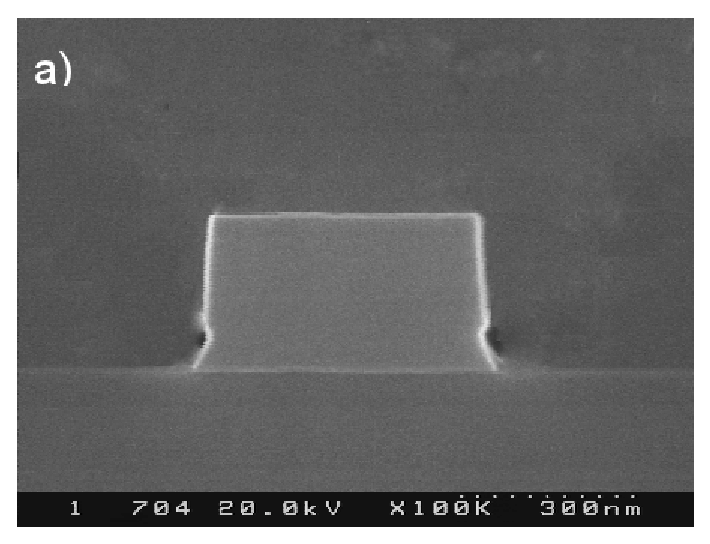
\includegraphics[width=0.325\textwidth]{p13_4}
    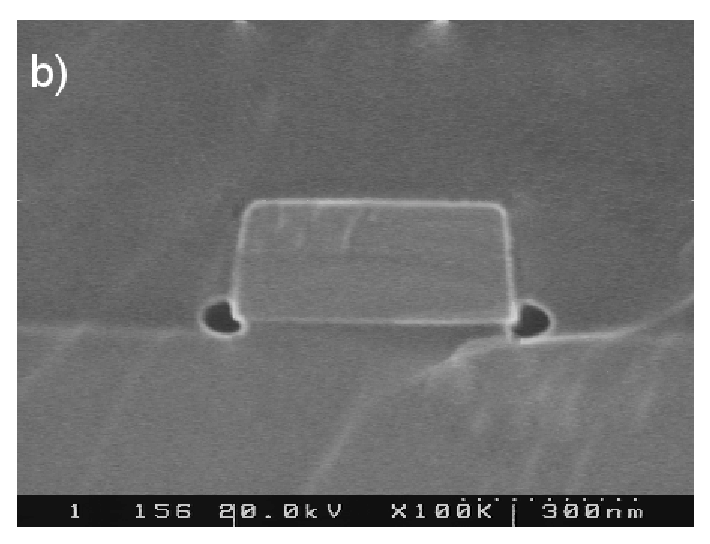
\includegraphics[width=0.325\textwidth]{semTM_4}
    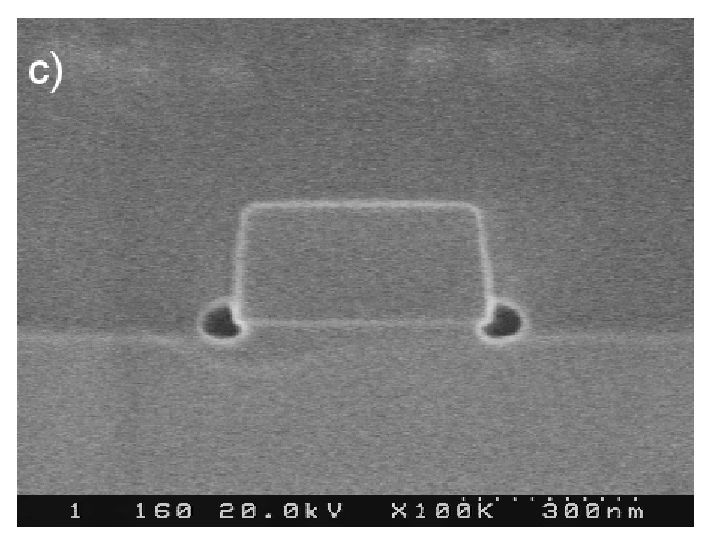
\includegraphics[width=0.325\textwidth]{semTE_2}
    \caption{SEM images of the amorphous silicon (a), TM SOI (b) and TE SOI (c). Air bubbles visible in the SOI samples were generated during facet preparation with HF to increase SEM contrast.}
    \label{fig:sem}
\end{figure}


%%%%%%%%%%%%%%%%%%%%%%%%%%
%%%%%%     Experiments      %%%%%%%%%%%
%%%%%%%%%%%%%%%%%%%%%%%%%%

\section{Four-wave-mixing: Re$\{ \gamma \}$}
Two continuous wave (cw) lasers were coupled to the waveguides, a pump beam with power $P_P(0)$ and a weaker signal beam with power $P_S(0)$, generating an idler signal at the waveguide output $P_i(L)$.
We measured the conversion efficiency as a function of the wavelength separation between pump and signal by using an optical spectrum analyzer (OSA) as shown in Fig.~\ref{fig:fwmOSA}.
Assuming that at these power levels (below 15~dBm) TPA is negligible, we can use Eq.~(\ref{eq:FWM}) as in Ref.~\cite{Vallaitis2009}.

%(Fig.~\ref{fig:fwmSetup}

%\begin{equation}
%       \eta ^2=\frac{\alpha_0^2}{\alpha_0^2+\Delta \beta^2}\left[ 1+ 4e^{-\alpha_0L}\frac{sin^2(L\Delta\beta/2)}{(1-e^{-\alpha_0L})^2} \right]
%\end{equation}

%where $ \Delta\beta $ for a detuning $ \Delta\lambda = \lambda_p-\lambda_s$ is given by:

%\begin{equation}
%       \Delta \beta=\frac{2\pi cD_2}{\lambda_p^2}\Delta\lambda^2
%\end{equation}



\begin{equation}
        P_i(L)=e^{-\alpha_0L}(\eta Re\{\gamma\}P_P(0)L_{eff})^2 P_s(0)
\label{eq:FWM}
\end{equation}


where $\alpha_0$ is the propagation loss, $L$ the waveguide total length, and $ L_{eff} $ the effective length, defined as $[ 1-\mathrm{exp}(-\alpha_0 L)] / \alpha_0 $

%where $\alpha_0$ is the propagation loss, $L$ the waveguide total length, and $ L_{eff} $ the effective waveguide length, which is defined as:
%\begin{equation}
        %L_{eff}=\frac{1-e^{-\alpha_0L}}{\alpha_0}
%\end{equation}

Finally, the conversion efficiency $\eta$ is given by \cite{Kung2003,Systems2004}:

\begin{equation}
        \eta ^2=\frac{\alpha_0^2}{\alpha_0^2+\Delta \beta^2}\left( 1+ 4e^{-\alpha_0L}\frac{sin^2(L\Delta\beta/2)}{1-e^{-\alpha_0L}} \right)
\end{equation}

where the phase mismatch for a detuning $ \Delta\lambda = \lambda_p-\lambda_s$ is

\begin{equation}
        \Delta \beta=\frac{2\pi cD_\lambda}{\lambda_p^2}\Delta\lambda^2
\end{equation}

where $D_\lambda$ is the chromatic dispersion parameter. One can relate the idler output to the signal output by rearranging Eq.~(\ref{eq:FWM}) obtaining

\begin{equation}
        \frac{P_i(L)}{P_s(L)}=(\eta Re\{\gamma\}P_P(0)L_{eff})^2 
\label{eq:ratio}
\end{equation}

which is the equation used for the calculation of $Re\{\gamma\}$ and dispersion $D_\lambda$ from the OSA spectra. Results are shown in Fig.~\ref{fig:fwmBw} and parameters of the fit are shown in Table~\ref{tab:resultsFOMpaper}.
The sign of the dispersion cannot be extracted from this method, but knowing the waveguide geometry, we calculated the dispersion of the waveguides using Finite Elements simulations.
We found a good fit with the numeric results shown in Table~\ref{tab:resultsFOMpaper} within a 10\% error, so this gave us the sign of dispersion. Dispersion of the SOI samples was also experimentally characterized with an interferometric setup obtaining a good agreement too \cite{Mas2012}.


%Moreover fitting the conversion bandwidth to equation~\ref{eq:ratio}
%\begin{figure}[htb]
 %  \centering
  %  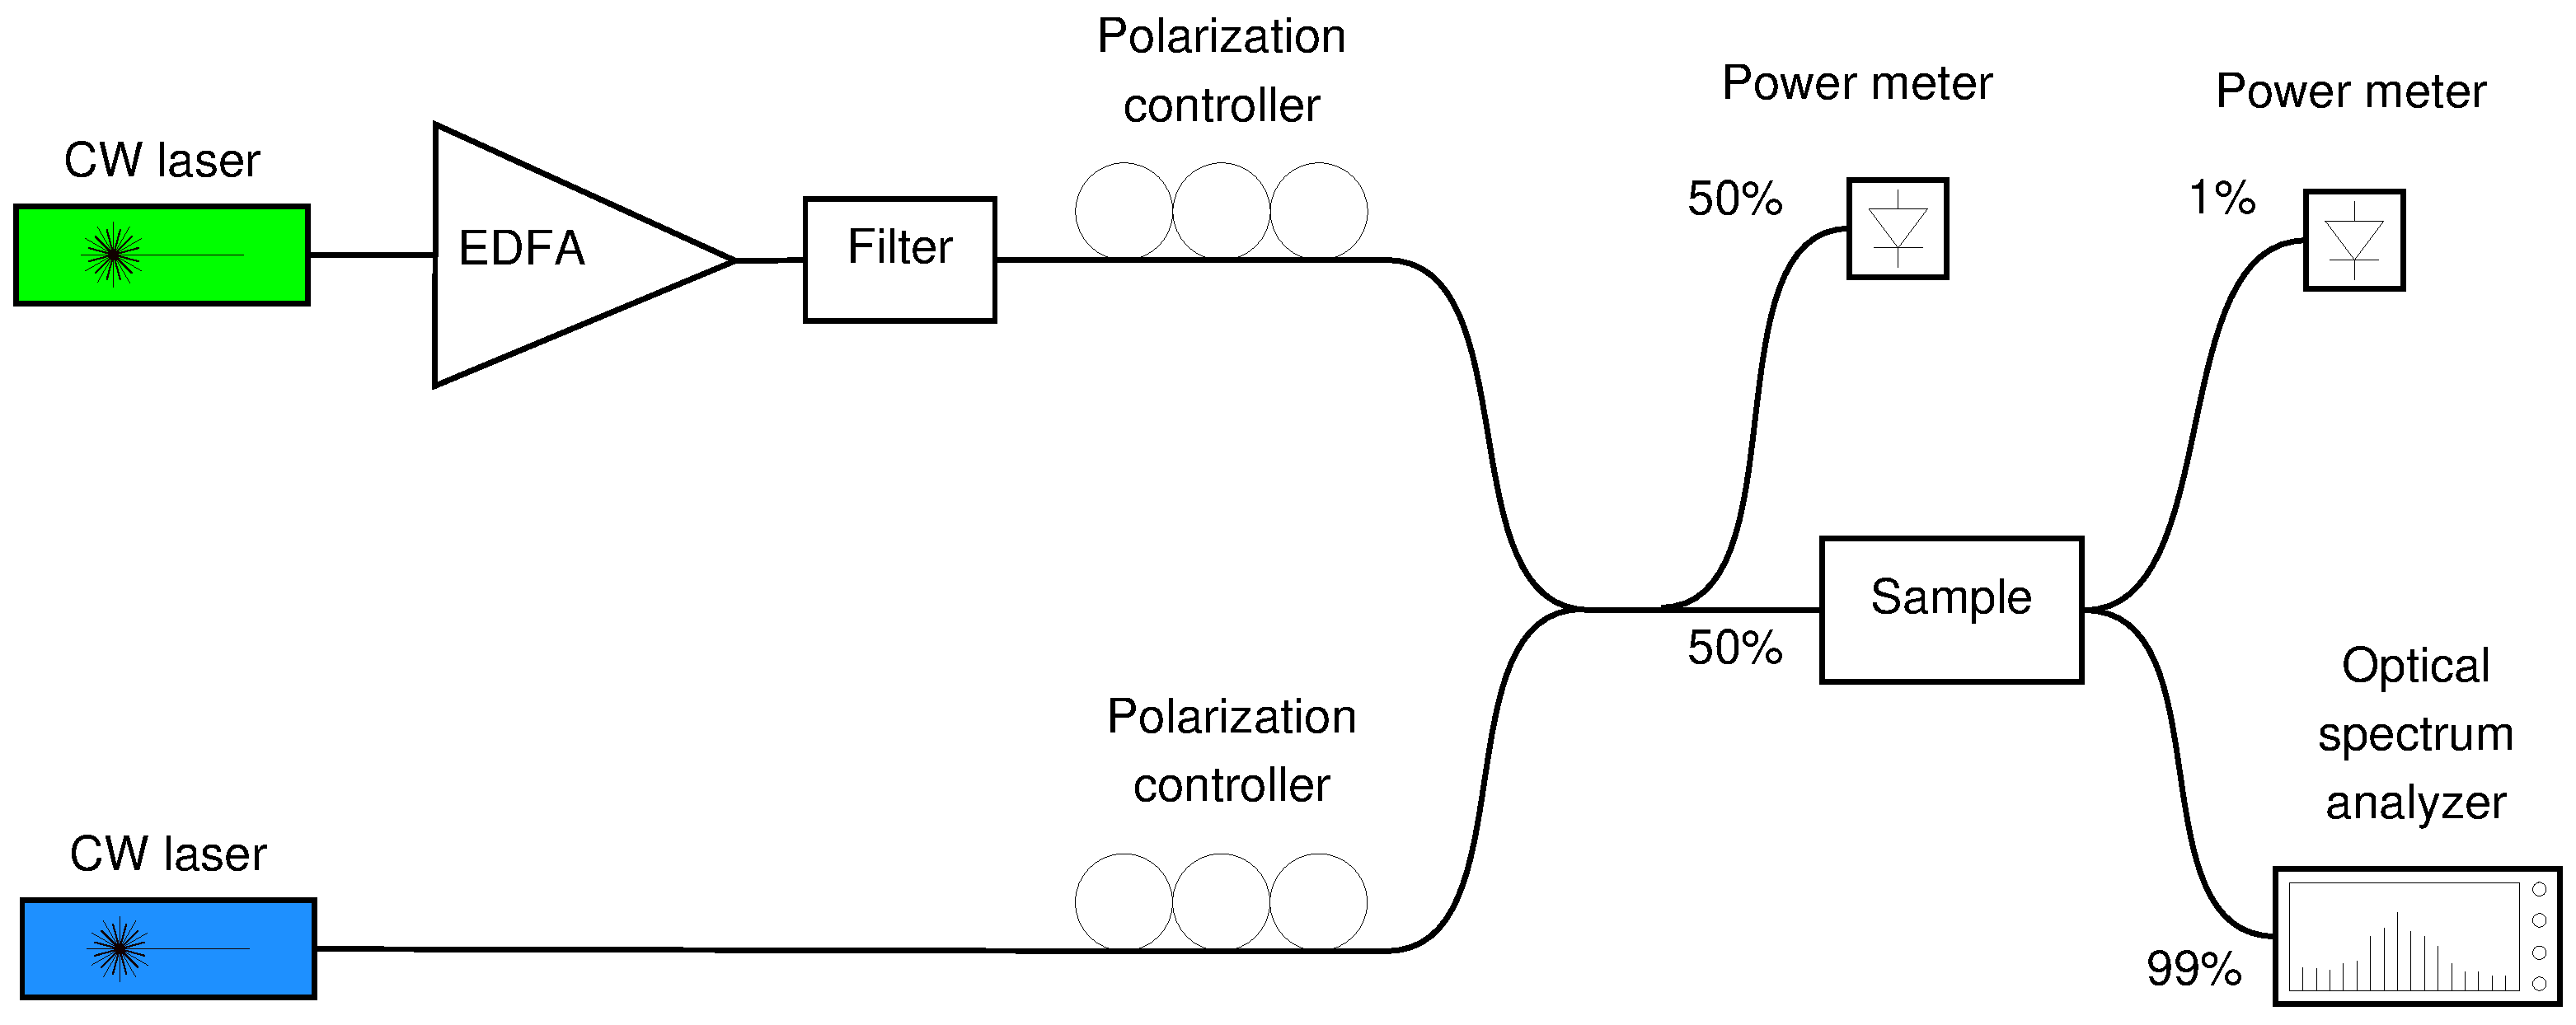
\includegraphics[width=1.00\textwidth]{fwmOneEdfa}s
   % \caption{Four Wave Mixing characterization setup.}
    %\label{fig:fwmSetup}
     %\end{figure}


\begin{figure}[htb]
    \centering
    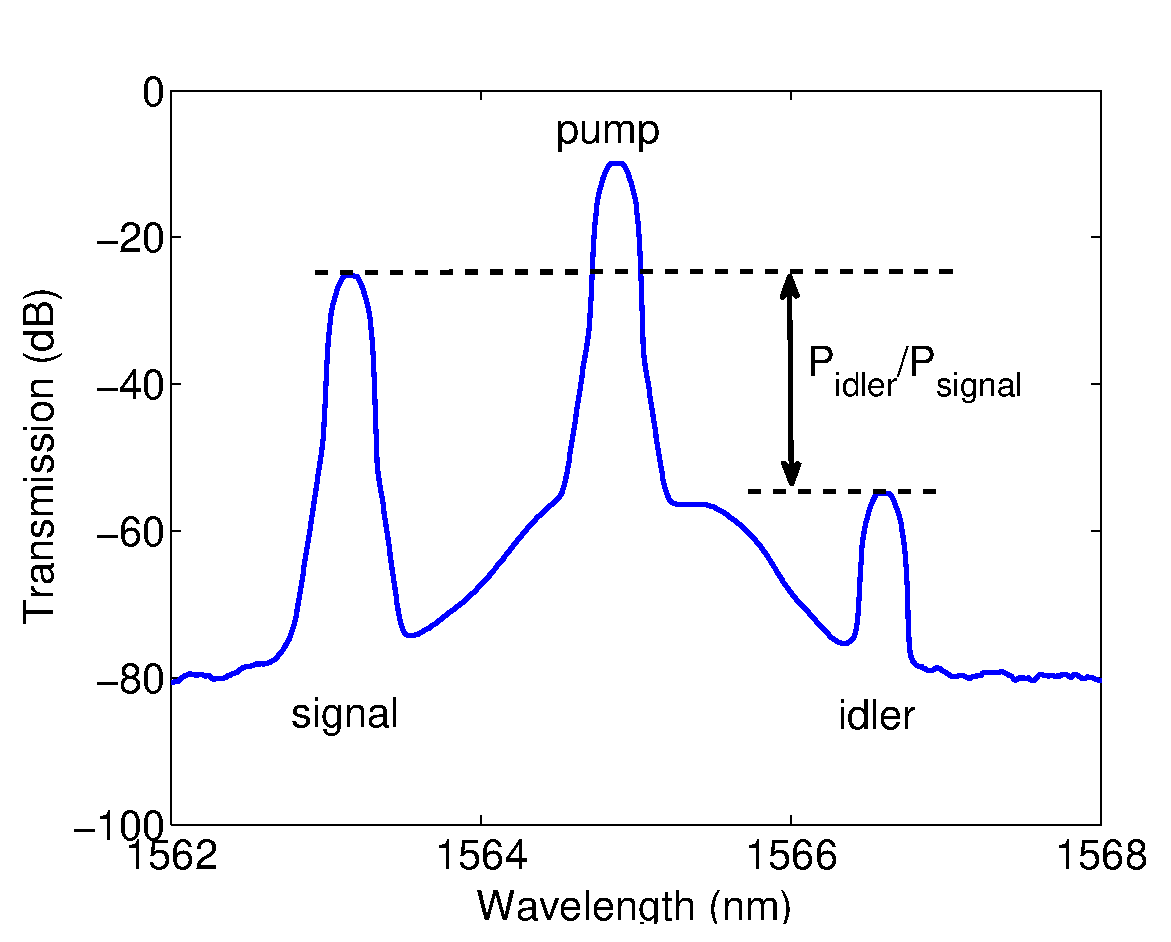
\includegraphics[width=0.45\textwidth]{Power_dBm_fwm_convEffMax_29p5dB}
    \caption{With 13~dBm pump power in waveguide a signal to idler conversion efficiency of -29.5~dB was measured in the FWM experiment.}
    \label{fig:fwmOSA}
\end{figure}
%Different signals in the FWM experiment. An idler with -29.5dB conversion efficiency was measure for 13dBm pump power in waveguide

\begin{figure}[htb]
    \centering
    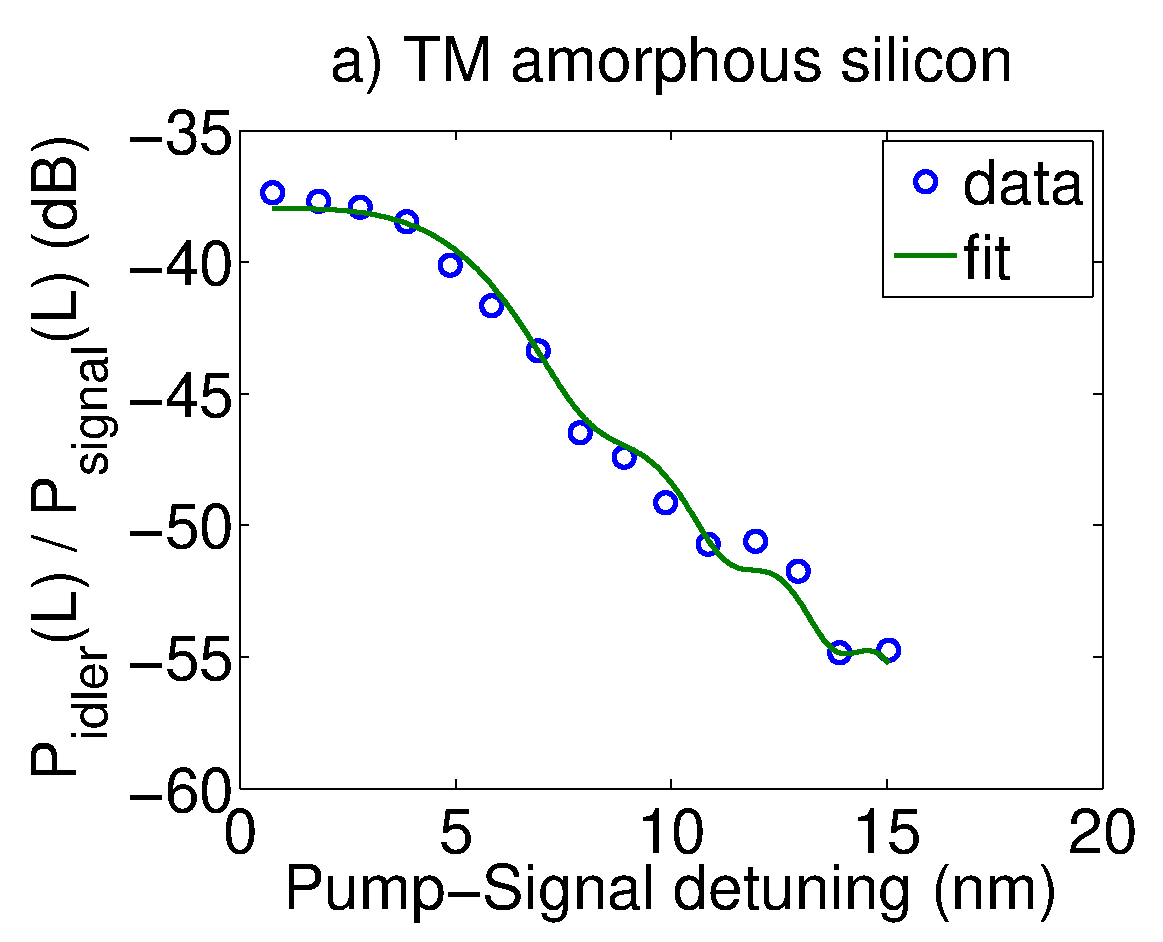
\includegraphics[width=0.32\textwidth]{fwm_bandwidth_P13_TM20mm_15dBmPump_6dBcm_332Wm_6474psKmnm_big_1pointMore}
    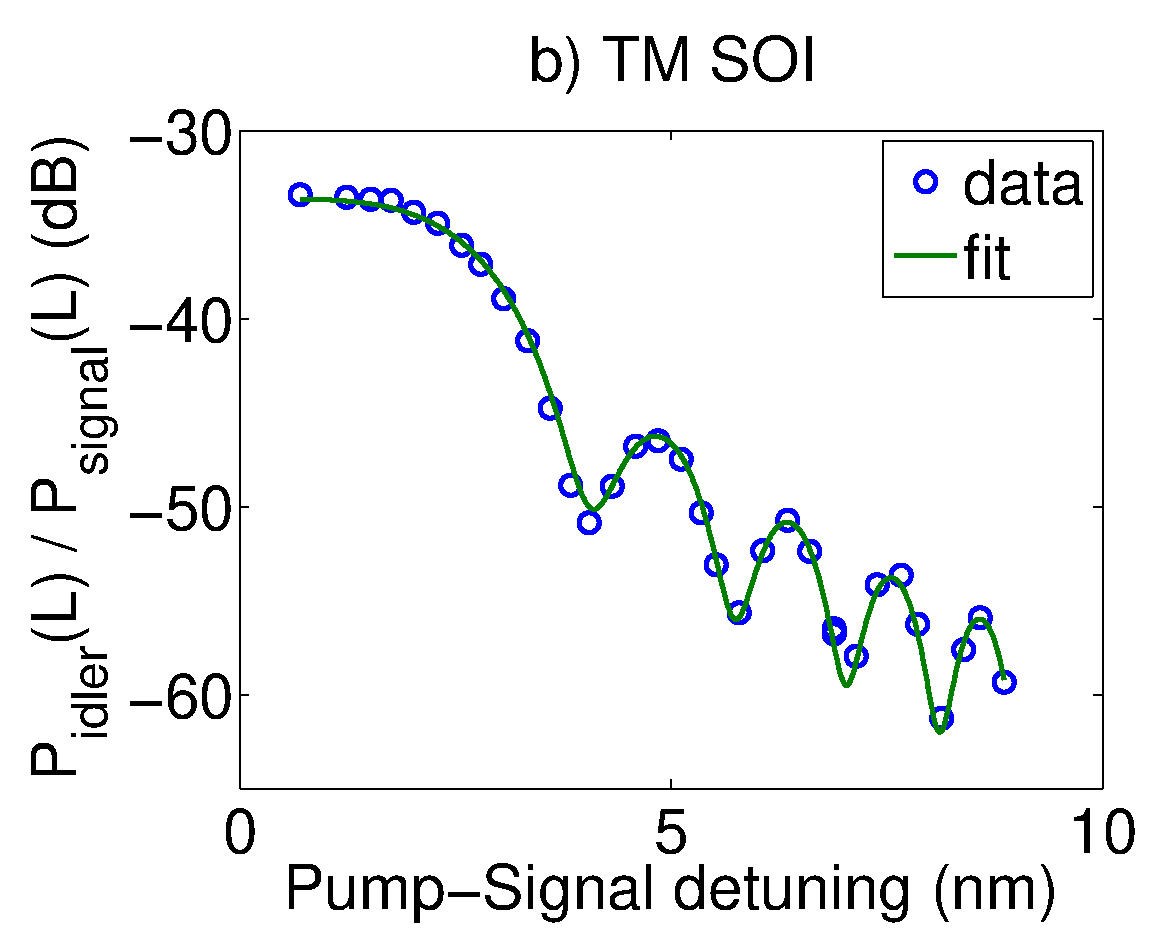
\includegraphics[width=0.32\textwidth]{fwm_bandwidth_V740_C11_TM25mm_20dBm_pump_1p67_46p81_19860psKmnm_big}
    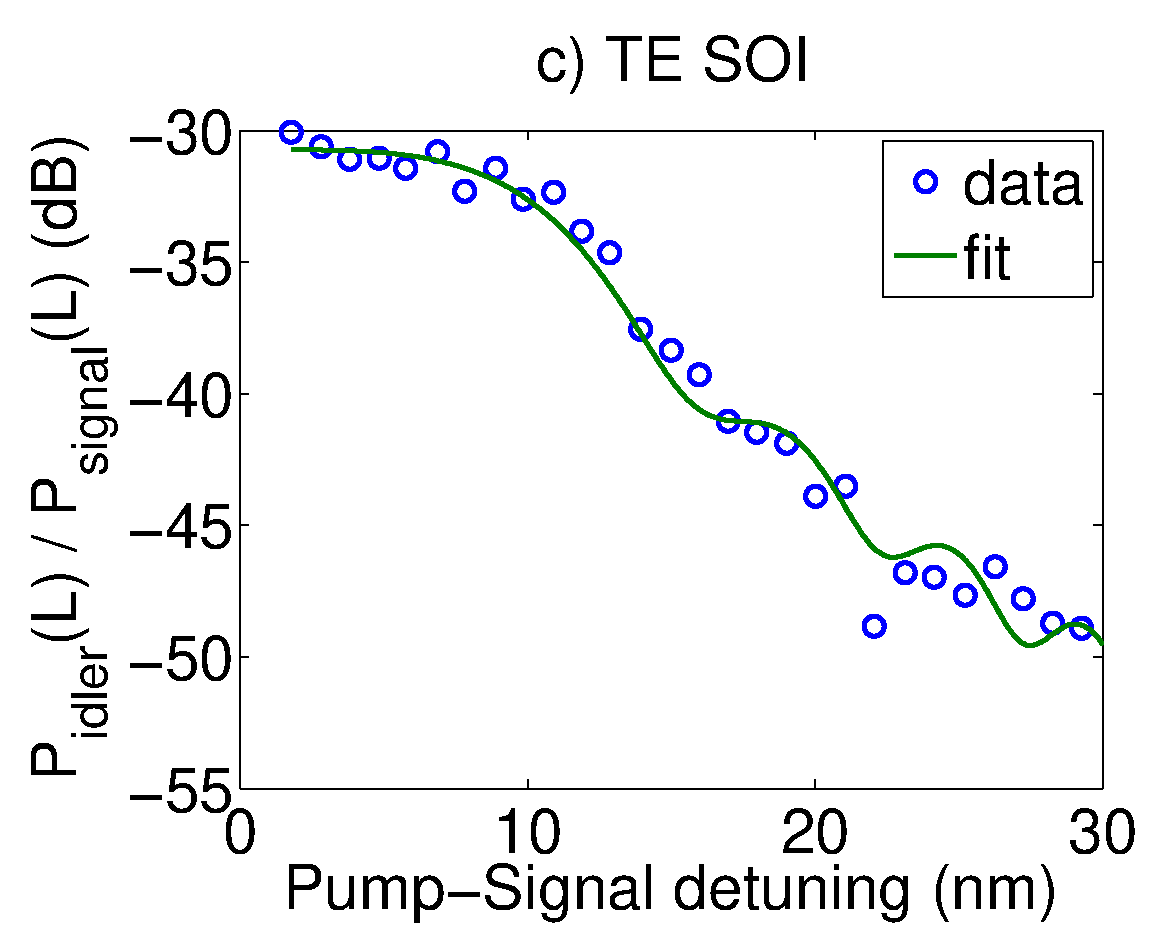
\includegraphics[width=0.32\textwidth]{fwm_BW_V740C11_TE25mm_15dBmPump_3p8dBcm_361Wm_-1322psKmnm_big}
    \caption{Four wave mixing conversion efficiency bandwidth. Pump power: 7.5~dBm (sample a), 14~dBm (sample b), 9~dBm (sample c). Dots are experimental points and the solid line is the fit to Eq.~(\ref{eq:ratio}).}
    \label{fig:fwmBw}
\end{figure}

We also show in Fig.~\ref{fig:fwmDifferentPump} the conversion efficiency for different input pump powers, where a slope very close to 2 was observed in all cases, confirming that the parametric conversion depends quadratically on the pump power.

\begin{figure}[htb]
    \centering
    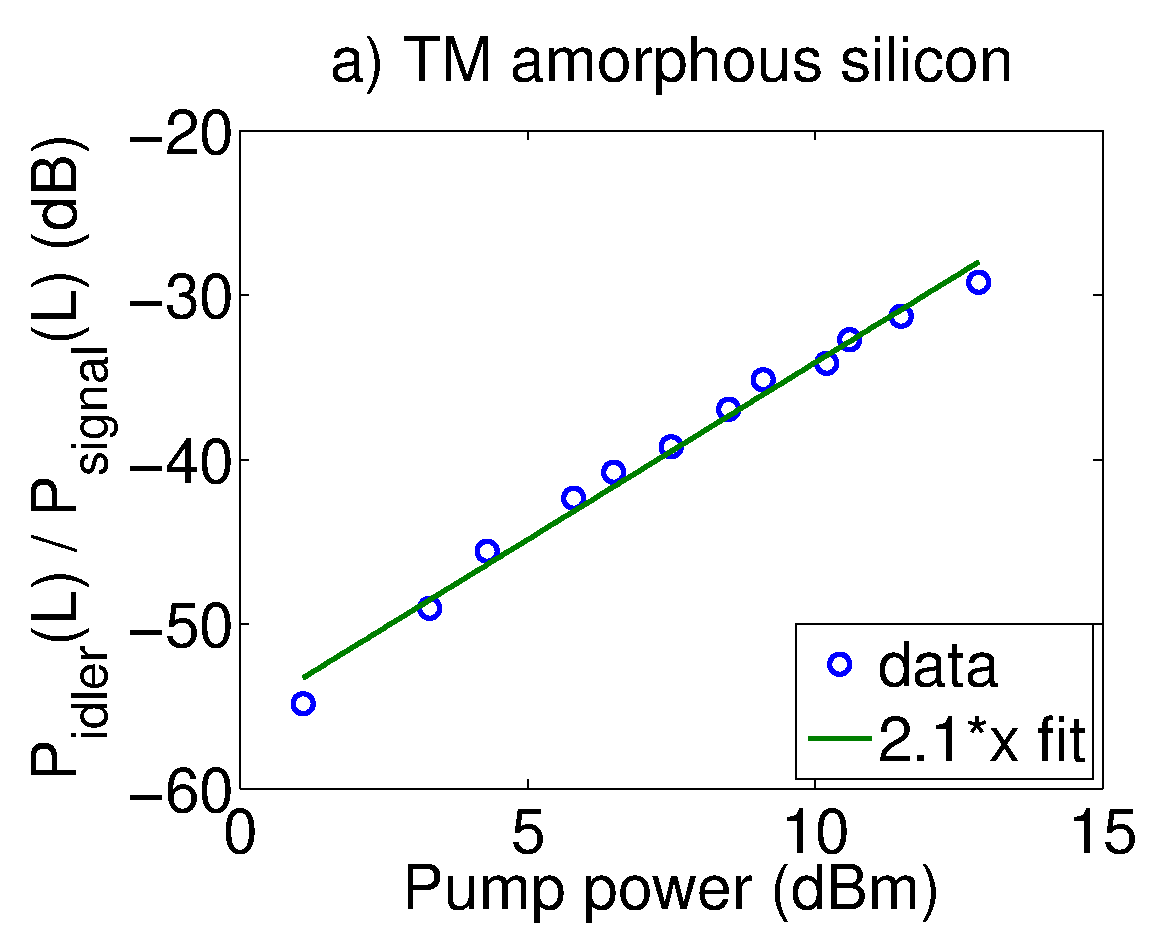
\includegraphics[width=0.32\textwidth]{fwm_differentPumps_aSitm20mm}
    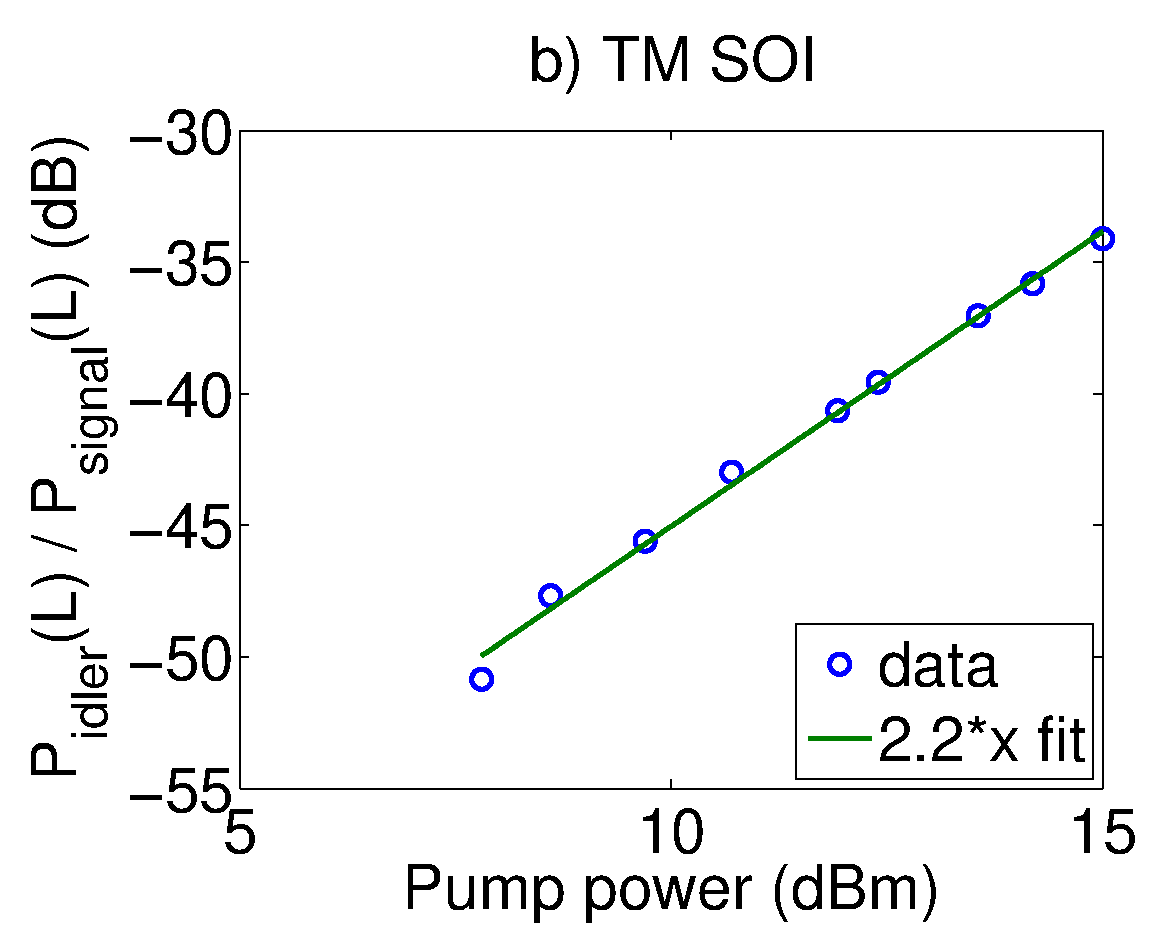
\includegraphics[width=0.32\textwidth]{fwm_differentPumps_tm}
    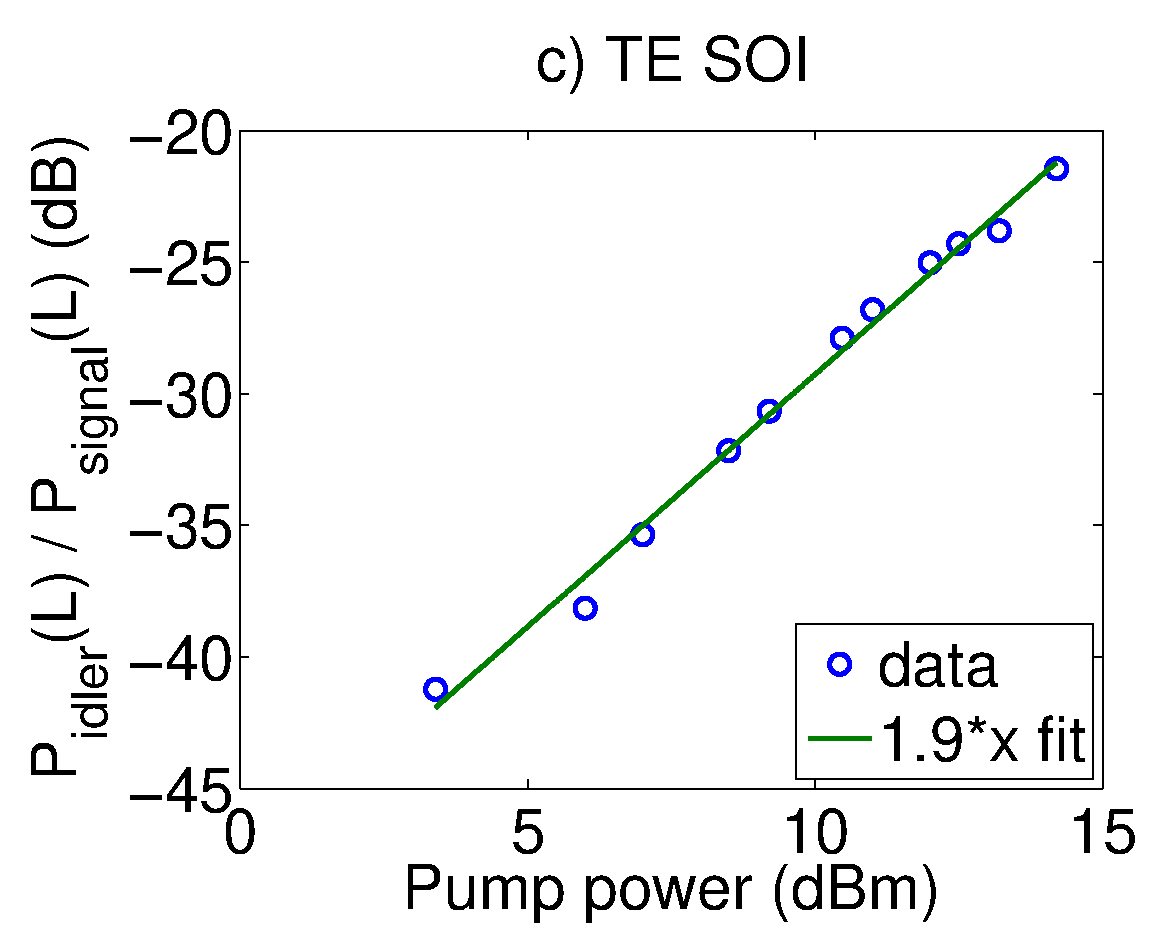
\includegraphics[width=0.32\textwidth]{fwm_differentPumps_te}
    \caption{Four wave conversion efficiency versus pump power. Dots: experimental points, solid line: linear fit. The slope of the linear fit in dB represents the power of the conversion efficiency versus pump power, which is close to 2 in all cases.}
    \label{fig:fwmDifferentPump}
\end{figure}






\section{Nonlinear loss measurements: Im\{$ \gamma $\}}
\label{sec:imGamma}
Two-photon absorption is a well-known process in silicon waveguides.
In a waveguide, we can consider it as the imaginary part of the gamma coefficient of the waveguide by using this differential equation:

\begin{equation}
 \frac{dP}{dz} = -\alpha_0 P(z) - 2|Im(\gamma)| P(z)^2 
\label{eq:differentialTPA}
\end{equation}

where P is the signal power through the waveguide, $\alpha$ is the linear loss of the waveguide, and $Im(\gamma)$ is the imaginary part of the $\gamma$ coefficient (we use the absolute value because we want to stress its loss character in the equation with a negative sign). 

The solution of the differential equation shown in Eq.~(\ref{eq:differentialTPA}) after a distance $L$ is given by:

\begin{equation}
 P(L) = \frac{e^{-\alpha_0 L}}{1+2|Im(\gamma)| L_{eff} P_0} P_0
\end{equation}

where $P_0$ is the input power in the waveguide. Therefore the ratio between the transmission at low power ($T_{LP} = e^{-\alpha_0 L} $) and the transmission at high power ($T_{HP} = P(L)/P_0 $) represents only the nonlinear loss $T_{NL}^{-1}$:

\begin{equation}
 T_{NL}^{-1} = \frac{T_{LP}}{T_{HP}} = 1+2|Im(\gamma)| L_{eff} P_0
\label{eq:transmissionLinear}
\end{equation}

which is a linear function on $P_0$.
The slope of the curve can give us the two-photon absorption coefficient of our waveguide as in \cite{Vallaitis2009}.
However, this equation is only valid for instantaneous transmission values.
When a pulsed signal is sent, and the transmission is averaged over time, the measured transmission would be the integral of the output, which we can define as:

%If one sends a pulsed signal, the equation is still correct for every instantaneous moment, but not correct for the overall transmission energy of the pulse.
%If one defines the energy transmission of a pulse $ \tilde{T} $ as the amount read by a power meter, one has to integrate the power along the whole pulse duration:

\begin{equation}
 \tilde{T}  = \frac{\int P(t,L)dt}{\int P_0(t)dt}
\end{equation}

where $\tilde{T}$ represent the averaged transmission of a pulsed signal with an input shape given by $P_0(t)$. With this definition, the ratio with the transmission at low power would be given by:


%\begin{equation}
 %\tilde{T} (L)^{-1} = \frac{\int P_0(t)dt}{\int P(t,L)dt} = \frac{\int P_0(t)dt} {e^{-\alpha L} \int \frac{P_0(t)}{1+2|Im(\gamma)| L_{eff} P_0(t)} dt}
%\end{equation}

\begin{equation}
\tilde{T}_{NL}^{-1} = \frac{\tilde{T}_{LP}}{\tilde{T}_{HP}} = \frac{\int P_0(t)dt}{\int \frac{P_0(t)}{1+2|Im(\gamma)| L_{eff} P_0(t)} dt}
\label{eq:transmissionIntegral}
\end{equation}


which depends on the actual pulse shape $P_{0}(t)$ that is introduced. If the pulsed signal has a rectangular shape, one can use Eq.~(\ref{eq:transmissionLinear}), but if the shape is different, the integral in Eq.~(\ref{eq:transmissionIntegral}) must be solved, as the result differs significantly.
The reason for this variation is the fact that the flanks of the pulse are not affected as hardly by TPA as the peak. Therefore, the overall energy transmission is higher than for the case of cw excitation.
For the particular case of a $sech^2$ shape, which corresponds to the output of our laser, the result of  Eq.~(\ref{eq:transmissionIntegral}) is given by:

% One can calculate analytically how much this transmission is for different typical pulse shapes.

%We assume a hyperbolic secant pulse, typical for solitons, which is the shape of our femtosecond fiber laser $  P_0(t) = P_{0 peak}~\mathrm{sech}^2 (\frac{t}{\tau}) $. Solving Eq.~(\ref{eq:transmissionIntegral}) for the hyperbolic secant is not trivial. After some algebraic manipulation and using some properties of inverse hyperbolic trigonometric functions, one can extract the analytical result, which is:<

%\begin{equation}
% P_0(t) = P_{0 peak}~sech^2 \frac{t}{\tau}
%\end{equation}



\begin{equation}
\tilde{T}_{NL}^{-1} = \frac{\tilde{T}_{LP}}{\tilde{T}_{HP}} \bigg|_{sech^2~shape}  = \frac{\sqrt{\delta}\sqrt{\delta + 1}}{\ln(\sqrt{\delta}+\sqrt{\delta+1})} ~~\mathrm{where}~~  \delta = 2|Im(\gamma)| L_{eff} P_{0 peak}
\label{eq:transmissionHypSecant}
\end{equation}

%for $ \delta = 2|Im(\gamma)| L_{eff} P_{0 peak} $

%\begin{figure}[htb]
 %   \centering
  %  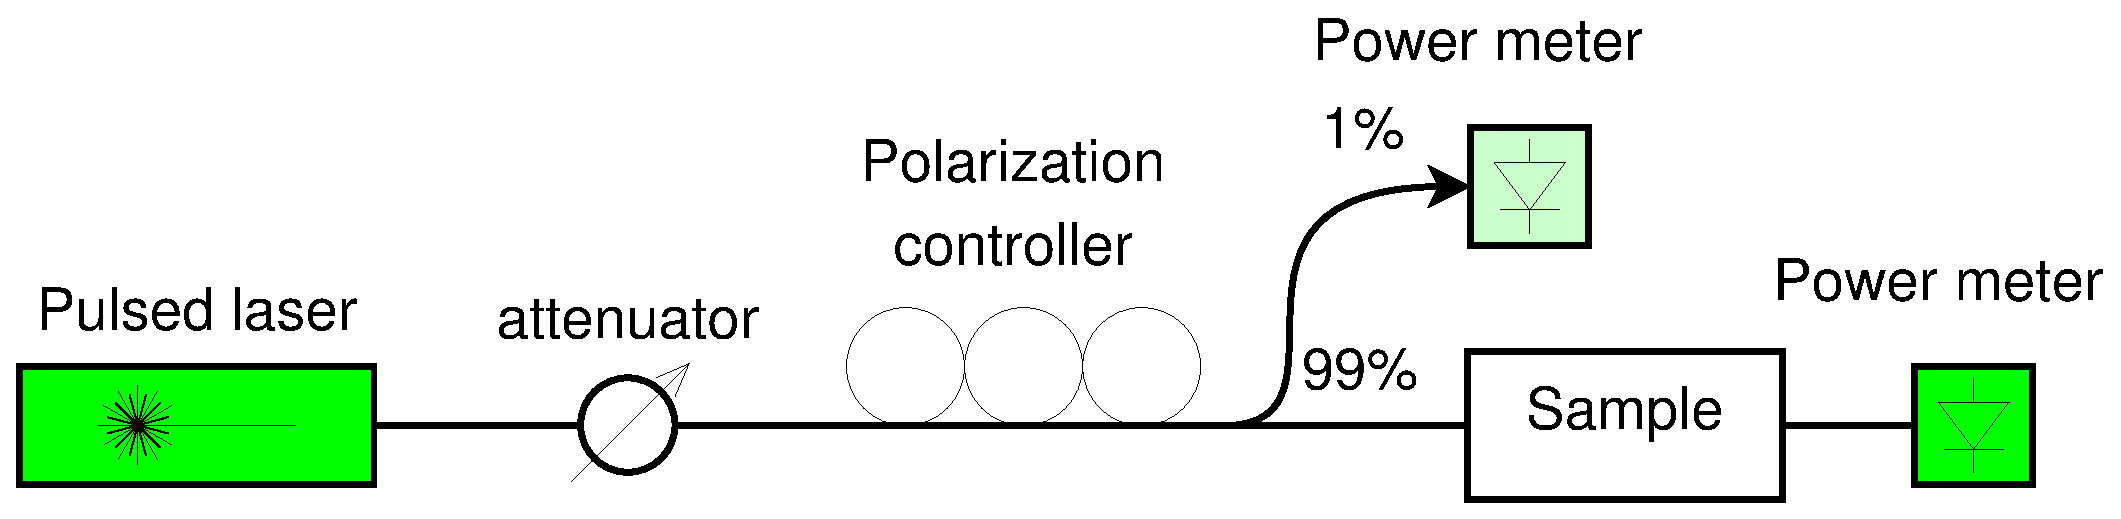
\includegraphics[width=1.0\textwidth]{imGammaFit}
   % \caption{Absorption characterization setup.}
    %\label{fig:setupImGamma}
%\end{figure}

We measured this parameter with a power meter using a picosecond laser at a wavelength of 1539~nm and a variable attenuator.
The results are shown in Fig.~\ref{fig:imGammaSamples}, where the curves were fitted to Eq.~(\ref{eq:transmissionHypSecant}) in order to extract the $Im(\gamma)$ parameter shown in Table~\ref{tab:resultsFOMpaper}.


%We measured the nonlinear loss with a power meter using a picosecond laser at a wavelength of 1539~nm and a variable attenuator. The results are shown in Fig.~\ref{fig:imGammaSamples}, where the curves were fitted to Eq.~\ref{eq:transmissionHypSecant} in order to extract the parameter $Im(\gamma)$ (see Table~\ref{tab:resultsFOMpaper}).

%In order to extract the $Im(\gamma)$ parameter, we measured the transmission for different peak powers using a picosecond laser at a wavelength of 1539~nm and a variable attenuator. The results substracting the linear loss (Fig.~\ref{fig:imGammaSamples}) were fitted to Eq.~\ref{eq:transmissionHypSecant} and shown in Table~\ref{tab:resultsFOMpaper}.


\begin{figure}[htb]
    \centering
    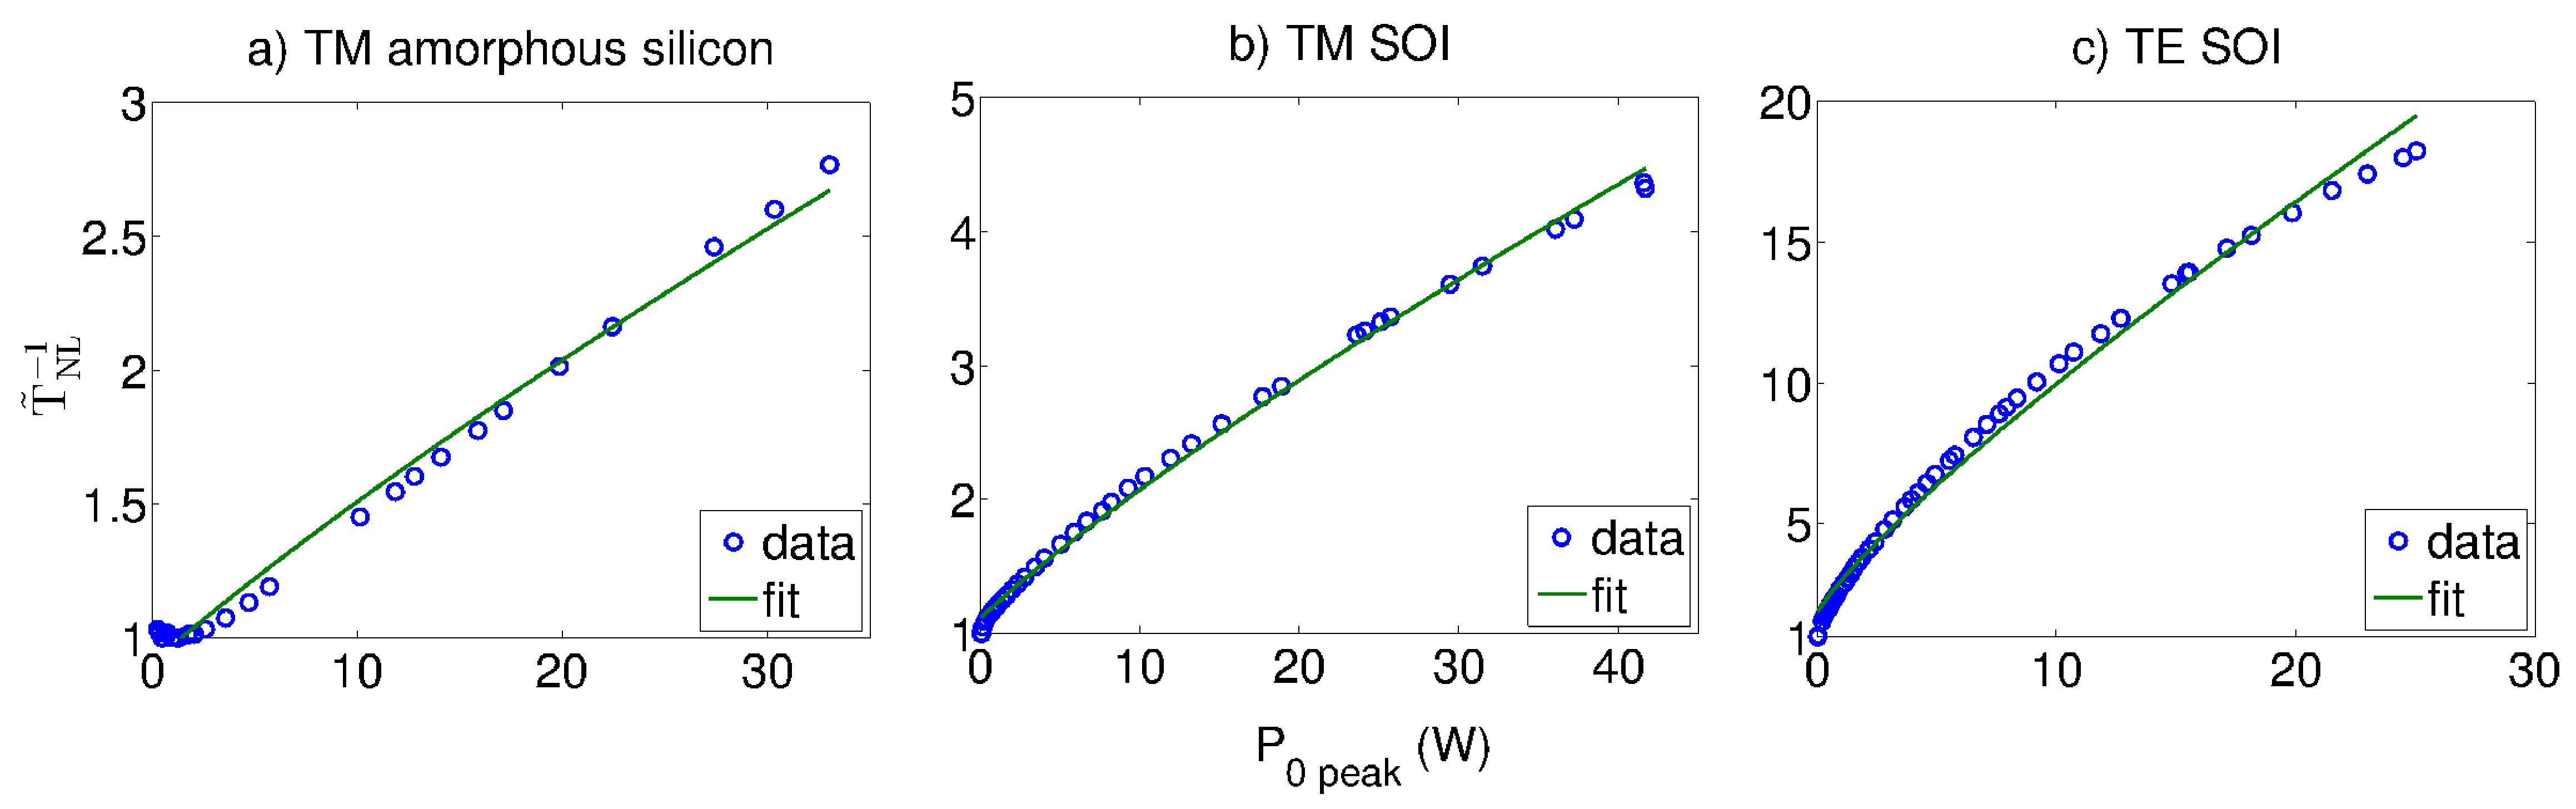
\includegraphics[width=1.0\textwidth]{imGamma_aSi_TM_TE}
      \caption{Transmission versus waveguide peak power (note the difference in the y-scale among the three plots). Solid line shows the fit for $ sech^2 $ pulses using Eq.~(\ref{eq:transmissionHypSecant}).}
    \label{fig:imGammaSamples}
\end{figure}



\section{Time-resolved measurements and simulations}
We characterize the samples with a time-resolved phase-sensitive technique similar to the one described in \cite{Vallaitis2008}.
The setup is shown in Fig.~\ref{fig:setupTimeRes}. In this technique, we divide a 1~ps laser pulse into three pulses, one of them intense (pump) and two identical weak ones (a reference and a probe).
Then we combine the pump very close to the probe, changing their separation with a variable delay line.
Finally the amplitude and phase of the probe is monitored as a function this delay by using a lock--in amplifier.

\begin{figure}[htb]
    \centering
    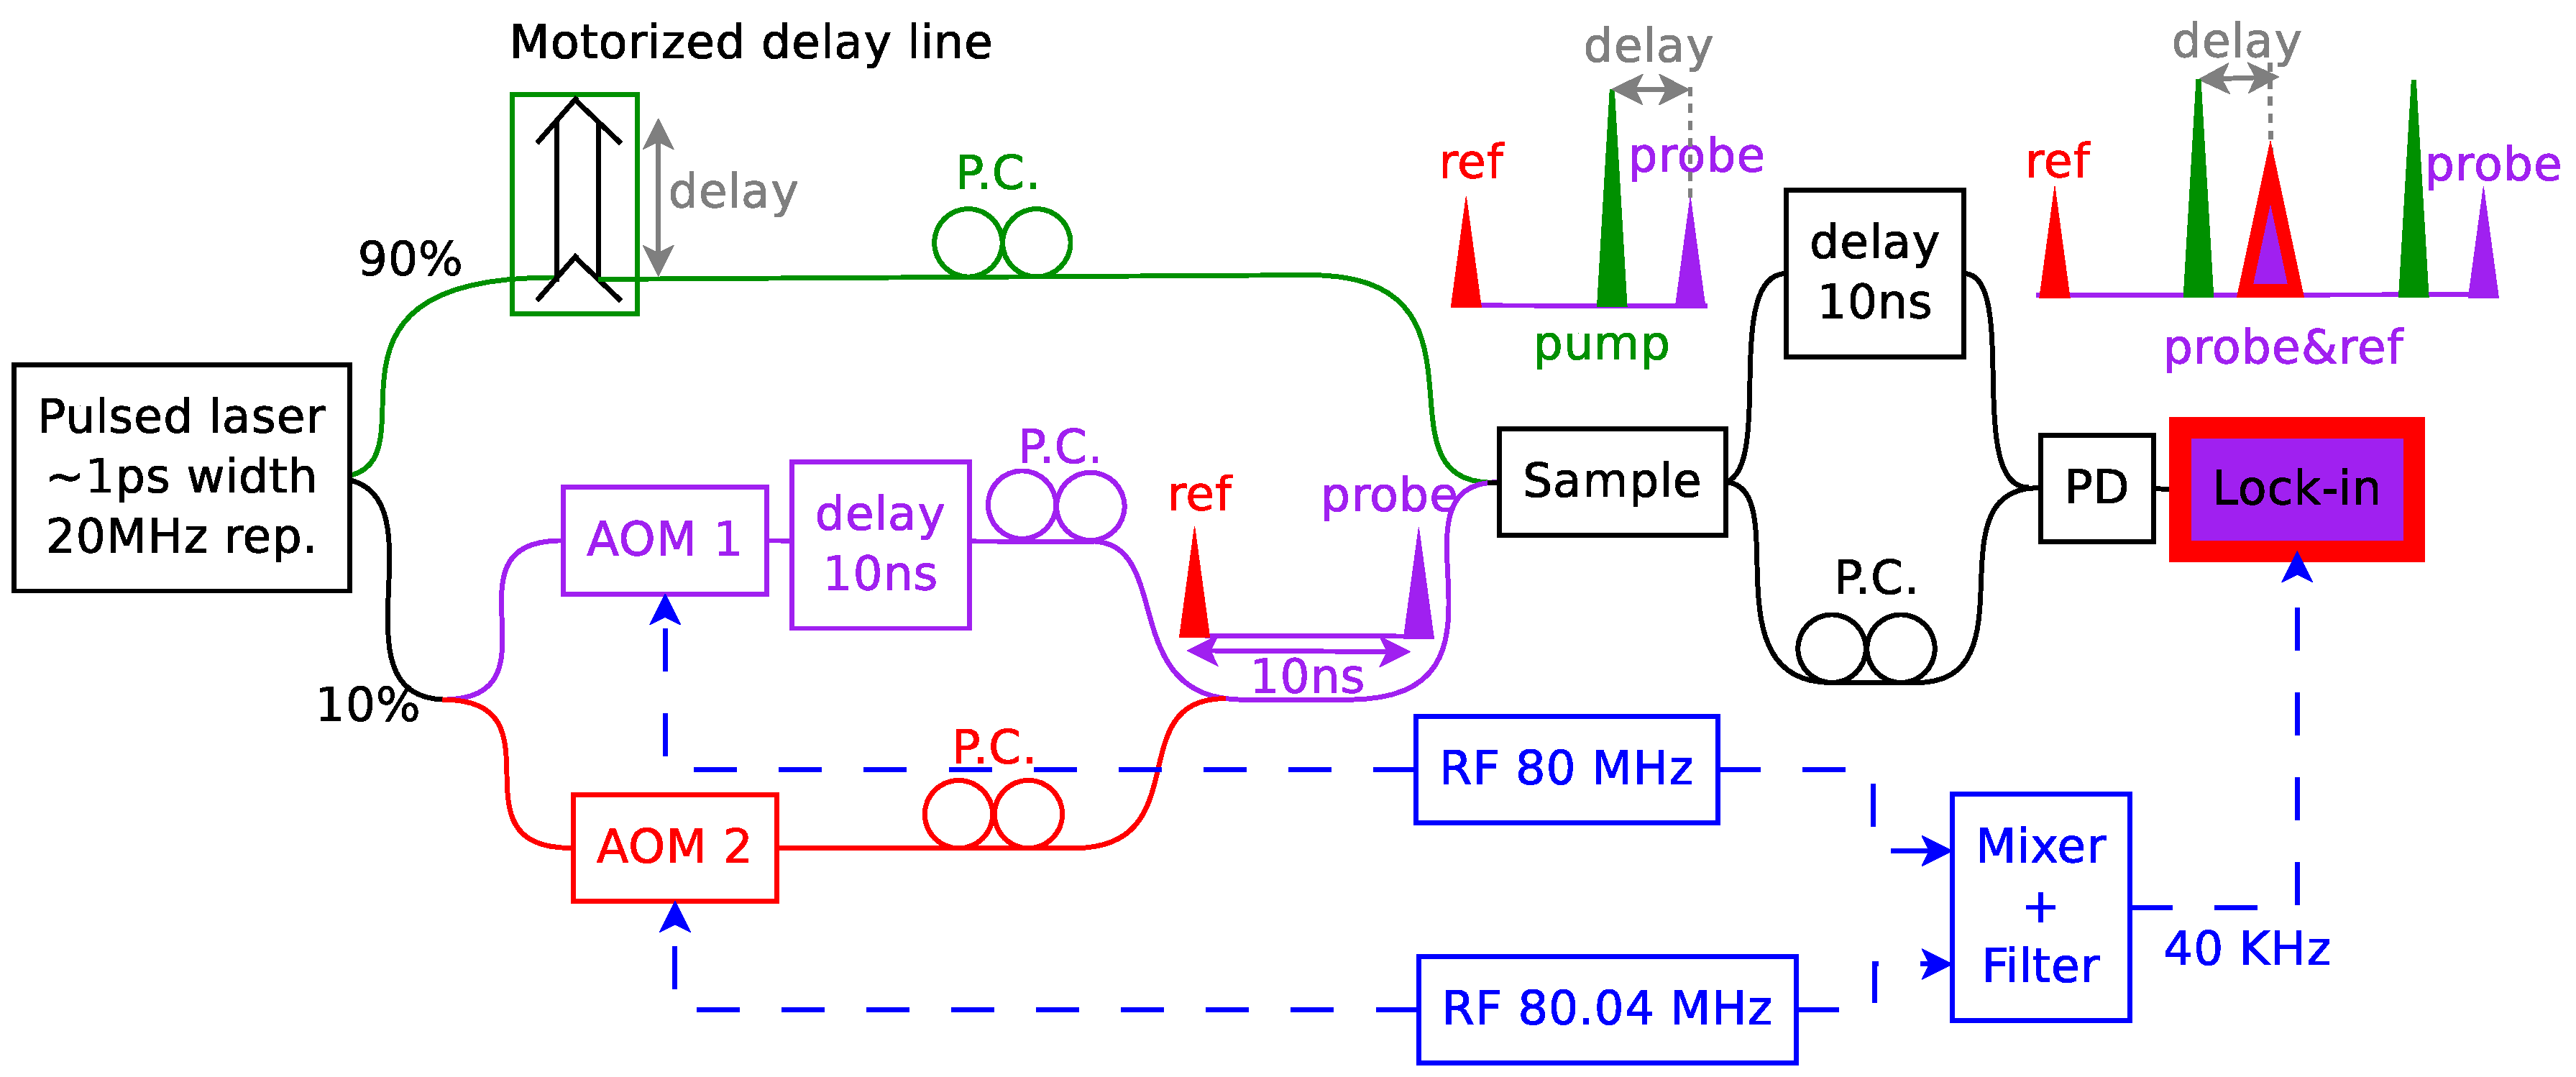
\includegraphics[width=1.0\textwidth]{timeResolved9}
    \caption{Time resolved characterization setup. PD: photodiode, PC: polarization controller, AOM: acousto-optic modulator.}
    \label{fig:setupTimeRes}
\end{figure}


In Fig. \ref{fig:timeResolvesMeasurements} we observe both Kerr and carrier effect in the TM amorphous silicon compared to SOI TM and TE strip waveguides.
They produce opposite phase shifts because Kerr produces an increase in refractive index ($ \Delta n > 0 $) and carriers decrease it ($ \Delta n < 0 $).
The dynamics of each of these processes is also very different. During the pump pulse, an instantaneous phase change is due to Kerr effect, together with an amplitude decrease.
his decrease is due to cross-absorption modulation (XAM), which consists of a two-photon absorption (TPA) process where one of the photons comes from the pump and the other one comes from the probe. Once the pump pulse is gone, in the SOI samples there is a phase response with opposite sign that remains for all the measurement range.
This is due to the carrier plasma effect, also known as free-carrier dispersion (FCD). 


The measurement of the amplitude attenuation due to XAM is affected by the artifact reported in \cite{Vallaitis2009}, where the abrupt phase changes create a frequency shift in the probe signal modifying the signal detected in the lock-in amplifier.

%For this reason, in order to obtain a reliable measurement of TPA, we performed nonlinear transmission experiments which are reported in section~\ref{sec:imGamma}.

\begin{figure}[htb]
    \centering
    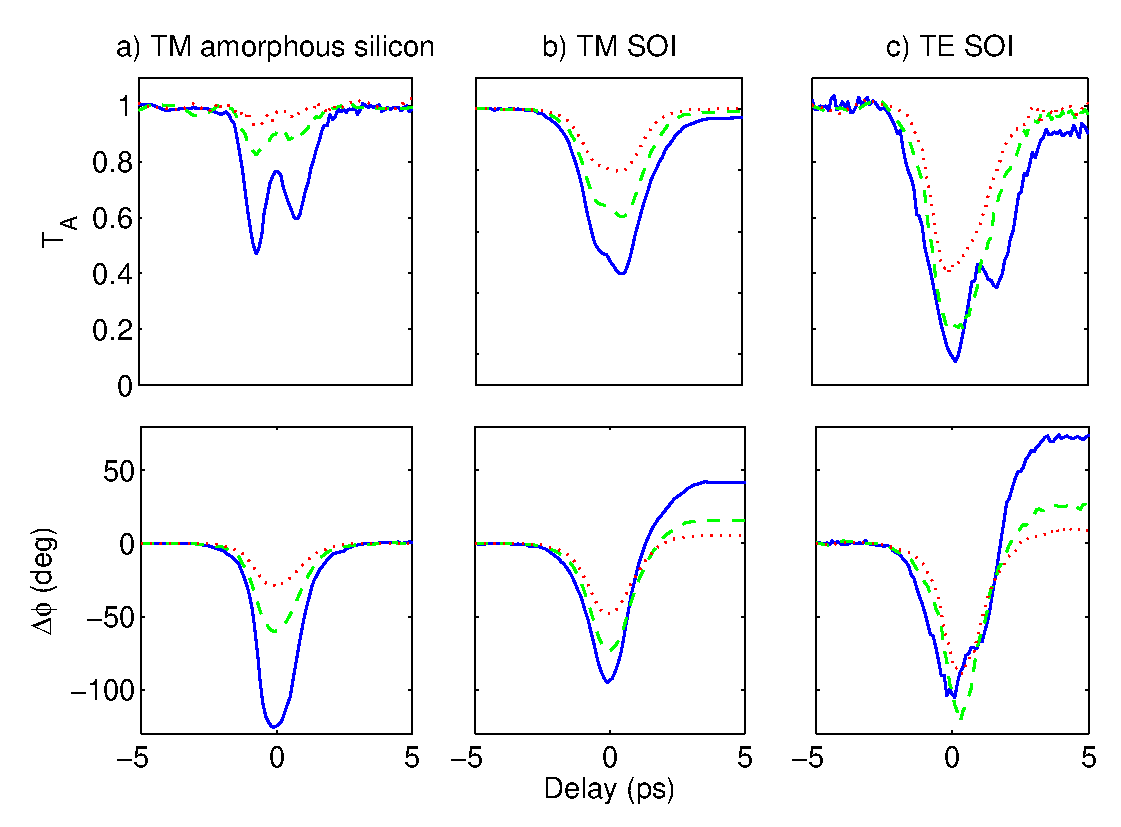
\includegraphics[width=1.00\textwidth]{timeResAmorfoTm10mmP13b_1w_0p5_0p25_0p125_amp_SOI_2}
    \caption{Time resolved measurements for different peak powers in waveguide. (sample a) 0.8W (---), 0.4W (-~-), 0.2W ($\cdot~\cdot$) (sample b) 6W (---), 3W (-~-), 1.5W ($\cdot~\cdot$) (sample c) 3W (---), 1.5W (-~-), 0.75W ($\cdot~\cdot$) }
    \label{fig:timeResolvesMeasurements}
\end{figure}



We used the nonlinear Schr\"{o}dinger equation to simulate the propagation of pump and probe pulses in optical waveguides, neglecting the Raman term, the self-steepening term and considering dispersion up to the second order \cite{Agrawal2001a}.
Solving the equation with the symmetrized split-step Fourier method as in \cite{Lin2007,Matres:12}, we cross-check simulations with experimental measurements in Figure~\ref{fig:timeResolvesSimulations}.
The output of the simulation is the envelope of the pump, probe and reference pulses, so in order to extract the output of the lock-in amplifier we calculated the overlap integral of the probe and reference pulses:


\begin{equation}
        |T_{A}|e^{j\phi} =
        \frac{\int E_{\mathrm{ref}}(\tau) E^*_{\mathrm{probe}}(\tau) ~ \mathrm{d}\tau}
        {\int |E_{\mathrm{ref}}(\tau)|^2~\mathrm{d}\tau}
\end{equation}


where $T_A$ and $\phi$ are respectively the transmitted amplitude and phase measured in the lock--in amplifier.


\begin{figure}[htb]
    \centering
    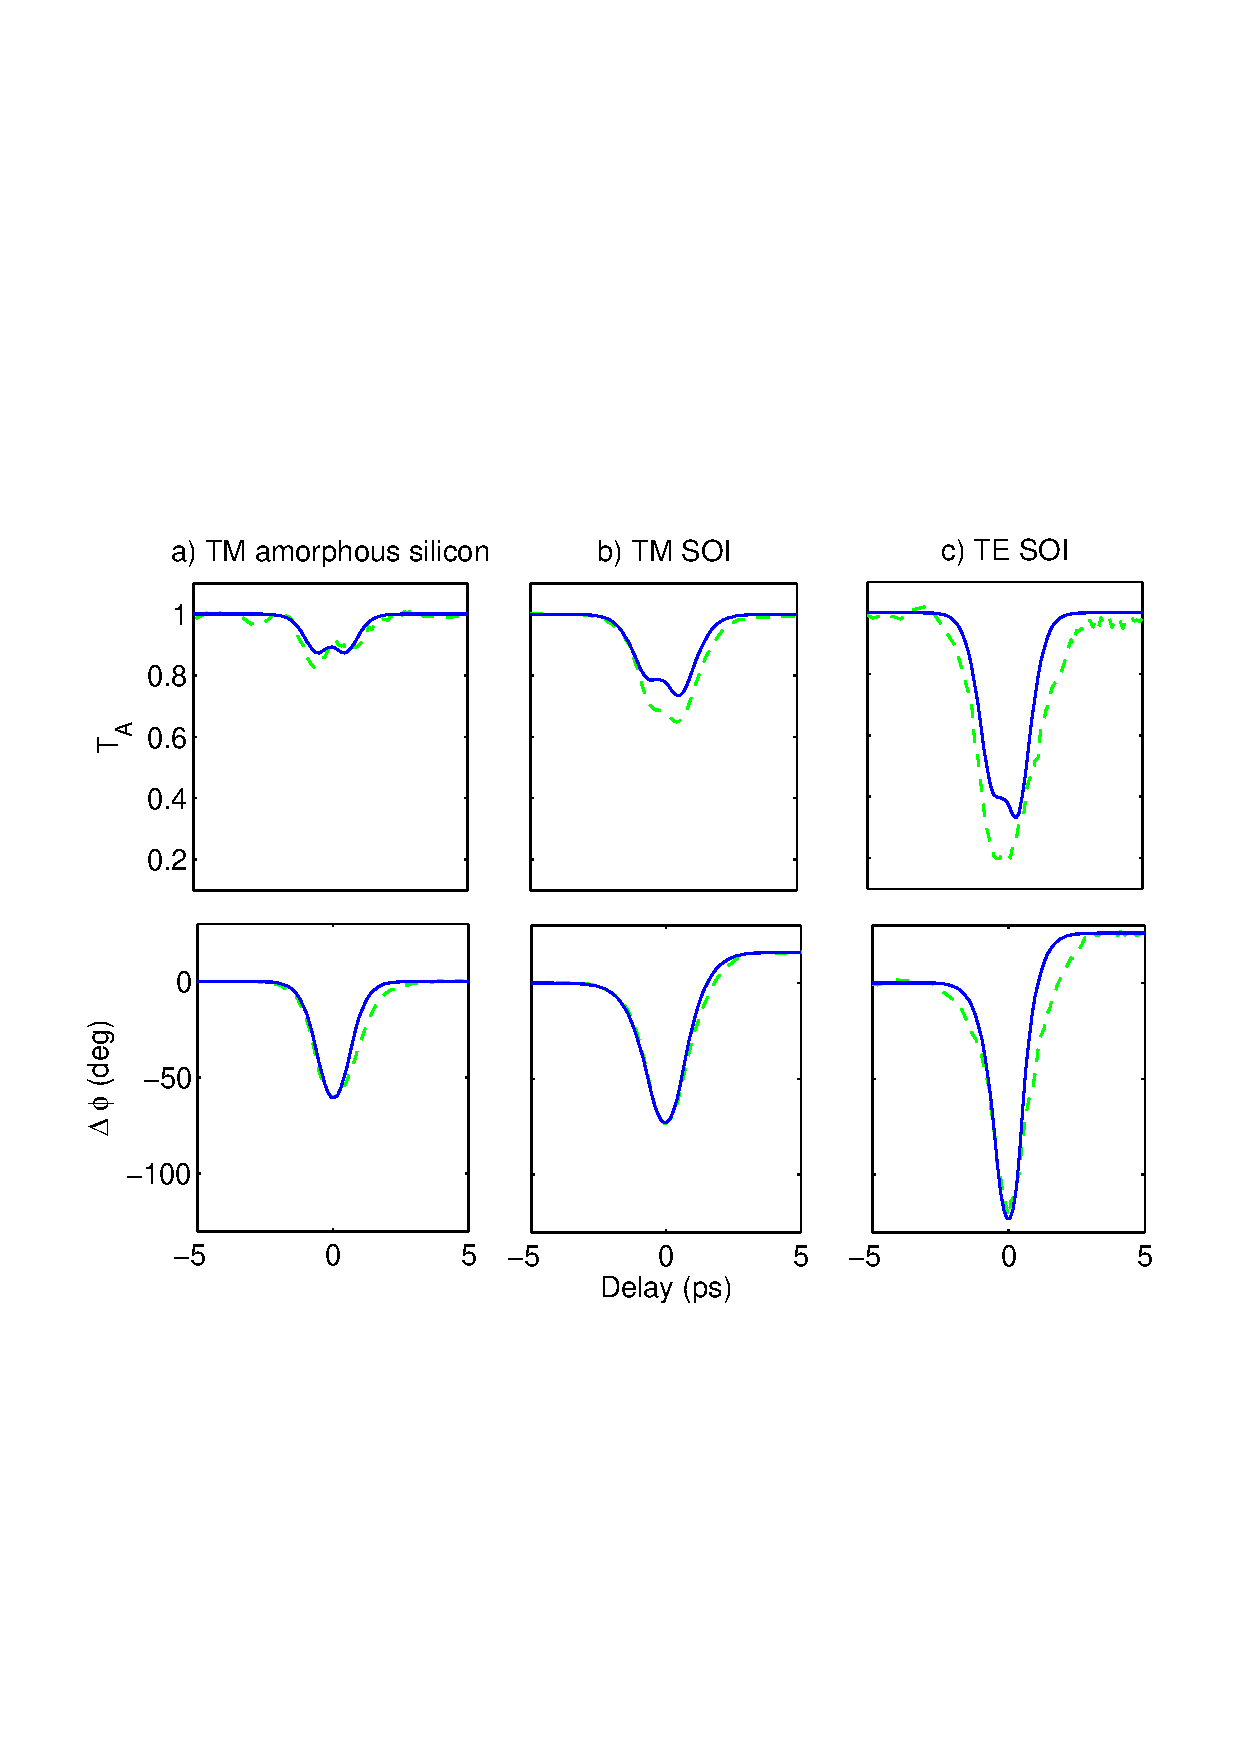
\includegraphics[width=1.00\textwidth]{timeRes_simulations_AmorfoTm10mmP13b_0p5w_SOI_2w__new}
    \caption{Time resolved measurements (-~-) and simulations (---) for 0.4W (sample a), 3W (sample b) and 1.5W (sample c) peak power in waveguide.}
    \label{fig:timeResolvesSimulations}
\end{figure}



\section{Results}

\begin{table}
\centering
\caption{Properties of the amorphous silicon waveguide compared with 445$\times$220~nm and 485$\times$220~nm (TE and TM) SOI waveguides.
The dispersion value was obtained through the fit of the FWM conversion bandwidth and its sign simulating the dispersion of the structure.
Figure of merit is defined as in paper~\cite{Koos2007} and ${A}_{eff}$ as in~\cite{Rukhlenko2012}.}
\begin{tabular}{l|ccc}
\hline
Sample & TM a-Si & TM SOI & TE SOI \\\hline
Coupling loss (dB) & 7.5 & 6 & 6\\
Propagation loss (dB/cm) & 4 & 1.9 & 4.9\\
$L_{eff}$ (mm) & 9.14 & 15.2 & 8.34\\
$D_\lambda$ (ps/(km$\cdot$ nm)) & -6500 & -19800 & -1200\\
$-\sigma_n ~ (10^{-21}~\mathrm{cm}^3) $  & \textless~1 & 10.7 & 13.8 \\ 
$ {A}_{eff}~ (\mathrm{\mu m}^2) $  & 0.21 & 0.33 & 0.13 \\ 
{$Re\{\gamma\} ~ (\mathrm{W}\cdot \mathrm{m})^{-1}$ } & 332 & 47 & 361\\
{$|Im\{\gamma\}| ~ (\mathrm{W}\cdot \mathrm{m})^{-1}$ } & 5.43 & 5.44 & 68.08\\
$ FOM = \frac{1}{4\pi} \frac{Re\{\gamma\}}{|Im\{\gamma\}|} $ & 4.9 & 0.69 & 0.43\\
\hline
\end{tabular}
\label{tab:resultsFOMpaper}
\end{table}

%effective FCD $ \frac{-\sigma_n}{ A_{eff} }~(10^{-15}~\mathrm{m}) $  & \textless~2 & 21 & 28 \\ 


Table~\ref{tab:resultsFOMpaper} shows all the numeric results of this work.
First, it is worth noting that the TM SOI sample is weakly confined in the vertical direction because the thickness is 220~nm, while confinement of the TM a-Si sample was considerably better, as the thickness was 250~nm.
This is the reason why both real and imaginary parts of $\gamma$ are much higher for TE SOI than for the TM SOI.
A similar behavior was reported in Ref.~\cite{Vallaitis2009}.
The FOM of the TM SOI (0.69) is also higher than the TE SOI (0.43) and higher than bulk silicon FOM (0.32) because there is more energy going through the silica cladding than for the TE SOI. On the other hand, the TM a-Si sample has a similar $Re\{\gamma\}$ than the TE SOI, but much lower $Im\{\gamma\}$, making the FOM several times higher.
The explanation of this, as claimed in the literature~\cite{Narayanan2010, Kuyken2011}, is the fact that a-Si has a higher band-gap, which makes TPA lower while keeping a similar Kerr coefficient.
The measured nonlinear coefficient $n_2$ in a-Si was $17.5 \cdot 10^{-5}\mathrm{cm}^2 / \mathrm{GW}$ which is 4.6 times higher than in the TM crystalline silicon SOI sample ($3.8 \cdot 10^{-5}\mathrm{cm}^2 / \mathrm{GW}$) while the $\beta_{TPA} $ was 1.5 times lower (0.23 in the a-Si versus 0.35 $\mathrm{cm} / \mathrm{GW}$).
Regarding the stability, we did not observe any degradation neither in the FWM conversion efficiency nor any change in the losses when using the pulsed laser at maximum power after one hour of operation, which means that the material is more stable than the one reported in Ref.~\cite{Kuyken2011}, which degraded significantly after few minutes of exposure.
The reason for this is probably differences in the fabrication conditions, and this is a topic under investigation but out of the scope of this work.

Time-resolved measurements show that the a-Si waveguide not only has a low TPA but also that free carriers have a negligible role. This is clear from Fig.~\ref{fig:timeResolvesMeasurements} where the phase curve does not have any slow component associated to the free carrier contribution. On the contrary, the response of strip waveguides shows a long tail with $\Delta n <0$ for delay times longer than 1~ns. This is confirmed by the FCD parameter ($\sigma_n$), defined in~\cite{Lin2007} and shown in Table~\ref{tab:resultsFOMpaper}. This feature would considerably reduce the undesired patterning effects when modulating a real bit pattern.

% (we have considered the effective FCD, which is normalized with the effective area, making it a device parameter like $\gamma$, rather than a material parameter)

Finally, the FOM reported in this work is also higher than the one shown in Refs.~\cite{Vallaitis2009,Koos2009} which was based on a hybrid waveguide with a nonlinear organic polymer in a slot configuration, yielding a FOM of 2.19. It is worth pointing out that amorphous Si is a more suitable material because it is CMOS compatible and less sensitive to temperature variations than organic materials.

\section{Conclusions}
We report nonlinear characterization of the real and imaginary parts of $\gamma$ of a-Si samples, and a comparison with SOI waveguides.
The measured FOM is 4.9, which is more than 7 times higher than for the SOI samples.  On the other hand, time-resolved experiments did not show any slow response associated with carriers. This material has the additional advantage that it can be grown at the back-end of CMOS line, unlike SOI.
These features make a-Si a suitable candidate for nonlinear all-optical switching applications.



\section*{Acknowledgments}
We acknowledge financial support from the Spanish Ministry of Science and Innovation SINADEC (TEC2008-06333) and PROMETEO/2010/087 NANOFOTONICA projects and Universidad Polit\'ecnica de Valencia for PAID2011/1914 and J. Matres' doctoral grant.

%\bibliographystyle{osajnl}
%\bibliography{library}
\bibliographystyle{unsrt}
\begin{thebibliography}{10}
\newcommand{\enquote}[1]{``#1''}


\bibitem{Almeida2004b}
V.~R. Almeida, C.~A. Barrios, R.~R. Panepucci, and M.~Lipson,
  \enquote{{All-optical control of light on a silicon chip.}} Nature
  \textbf{431}, 1081--1084 (2004).

\bibitem{Lee2009}
B.~G. Lee, A.~Biberman, A.~C. Turner-Foster, M.~A. Foster, M.~Lipson, A.~L.
  Gaeta, and K.~Bergman, \enquote{{Demonstration of broadband wavelength
  conversion at 40 Gb/s in silicon waveguides},} IEEE Photon. Technol. Lett. \textbf{21}, 182--184 (2009).

\bibitem{Kuyken2011a}
B.~Kuyken, S.~K. Selvaraja, W.~Bogaerts, D.~Van, P.~Emplit, S.~Massar,
  G.~Roelkens, and R.~Baets, \enquote{{On-chip parametric amplification with 26.5~dB gain at telecommunication wavelengths using CMOS-compatible hydrogenated amorphous silicon waveguides},} Opt. Lett.  36, 552-554 (2011).

\bibitem{Mizrahi1989}
V.~Mizrahi, K.~W. Delong, G.~I. Stegeman, M.~A. Saifi, and M.~J. Andrejco,
  \enquote{{Two-photon absorption as a limitation to all-optical switching.}}
  Opt. Lett. \textbf{14}, 1140--1142 (1989).

\bibitem{Narayanan2010}
K.~Narayanan and S.~F. Preble, \enquote{{Optical nonlinearities in
  hydrogenated-amorphous silicon waveguides.}} Opt. Express \textbf{18},
  8998--9005 (2010).

\bibitem{OLeary1997}
S.~K. O’Leary, S.~R. Johnson, and P.~K. Lim, \enquote{{The relationship
  between the distribution of electronic states and the optical absorption
  spectrum of an amorphous semiconductor: An empirical analysis},} J. Appl. Phys. \textbf{82}, 3334 (1997).

\bibitem{Kuyken2011}
B.~Kuyken, H.~Ji, S.~Clemmen, S.~K. Selvaraja, H.~Hu, M.~Pu, M.~Galili,
  P.~Jeppesen, G.~Morthier, S.~Massar, L.~K. Oxenl\o~we, G.~Roelkens, and
  R.~Baets, \enquote{{Nonlinear properties of and nonlinear processing in
  hydrogenated amorphous silicon waveguides.}} Opt. Express \textbf{19},
  B146--153 (2011).

\bibitem{Vallaitis2009}
T.~Vallaitis, S.~Bogatscher, L.~Alloatti, P.~Dumon, R.~Baets, M.~L. Scimeca,
  I.~Biaggio, F.~Diederich, C.~Koos, W.~Freude, and J.~Leuthold,
  \enquote{{Optical properties of highly nonlinear silicon-organic hybrid (SOH)
  waveguide geometries.}} Opt. Express \textbf{17}, 17357--17368 (2009).

\bibitem{Kung2003}
T. Kung, C. Chang, J. Dung, and S. Chi, \enquote{{Four-wave mixing between pump and signal in a distributed
  Raman amplifier},}  J. Lightwave Technol. \textbf{21}, 1164-1170 (2003).


\bibitem{Systems2004}
M.~Wu, and W.~I. Way, \enquote{{Fiber Nonlinearity Limitations in Ultra-Dense WDM Systems},} J. Lightwave Technol. \textbf{22}, 1483--1498 (2004).


\bibitem{Mas2012}
S.~Mas, J.~Matres, J.~Mart\'i, and C.~J. Oton, \enquote{{Accurate chromatic
  dispersion characterization of photonic integrated circuits},} IEEE Photon. J. \textbf{4}, 825--831 (2012).


\bibitem{Vallaitis2008}
T.~Vallaitis, C.~Koos, R.~Bonk, W.~Freude, M.~Laemmlin, C.~Meuer, D.~Bimberg,
  and J.~Leuthold, \enquote{{Slow and fast dynamics of gain and phase in a
  quantum dot semiconductor optical amplifier.}} Opt. Express \textbf{16},
  170--178 (2008).

\bibitem{Agrawal2001a}
G.~P. Agrawal, \emph{{Nonlinear Fiber Optics}}, (Academic Press, 2001).

\bibitem{Lin2007}
Q.~Lin, O.~J. Painter, and G.~P. Agrawal, \enquote{{Nonlinear optical phenomena
  in silicon waveguides: modeling and applications.}} Opt. Express
  \textbf{15}, 16604--16644 (2007).

\bibitem{Matres:12}
J.~Matres, C.~Lacava, G.~C. Ballesteros, P.~Minzioni, I.~Cristiani, J.~M.
  F\'{e}d\'{e}li, J.~Mart\'i, and C.~J. Oton, \enquote{{Low TPA and
  free-carrier effects in silicon nanocrystal-based horizontal slot
  waveguides},} Opt. Express \textbf{20}, 23838--23845 (2012).

\bibitem{Koos2007}
C.~Koos, L.~Jacome, C.~Poulton, J.~Leuthold, and W.~Freude, \enquote{{Nonlinear
  silicon-on-insulator waveguides for all-optical signal processing.}} Opt. Express \textbf{15}, 5976--5990 (2007).

\bibitem{Rukhlenko2012}
I.~D. Rukhlenko, M.~Premaratne, and G.~P. Agrawal, \enquote{{Effective mode
  area and its optimization in silicon-nanocrystal waveguides.}} Opt. Lett.
  \textbf{37}, 2295--2297 (2012).

\bibitem{Koos2009}
C.~Koos, P.~Vorreau, T.~Vallaitis, P.~Dumon, W.~Bogaerts, R.~Baets,
  B.~Esembeson, I.~Biaggio, T.~Michinobu, F.~Diederich, W.~Freude, and
  J.~Leuthold, \enquote{{All-optical high-speed signal processing with silicon
  – organic hybrid slot waveguides},} Nature Photonics \textbf{3}, 1--4
  (2009).

\end{thebibliography}
